\section{Wupper package}

In this section, the firmware, drivers, and tools of Wupper together with its working principle are explained. 

\begin{figure}[H]
	\centering
	\includegraphics[width = 0.8 \textwidth]{figures/full_application_structure.pdf}	
	\caption{Overview of the HDL modules in the Wupper package}
	\label{fig:wupperpackage}
\end{figure}


\subsection {Wupper core}
A DMA Engine, like Wupper, moves data bidirectionally to a memory buffer without CPU intervention. This efficient method is used for handling large amounts of data, which is crucial for throughput intensive applications. During a DMA tranfer, the DMA control core will take control according to the information provided by a DMA descriptor, and by flagging completion of operations in a per descriptor status register. By providing user data into the FIFO's, the core starts the DMA transfer over the PCIe lanes. Figure~\ref{fig:wupperpackage} shows a simplified diagram of the of the HDL modules of the Wupper package; including the HDL modules for the Wupper core and the example application, together with the host PC memory. Figure ~\ref{fig:pcie_core_structure} shows a more detailed block diagram of the Wupper core.
\newpage

\begin{figure}[H]
	\centering
	\includegraphics[trim=0mm 0cm 0mm 1cm,width=0.75\textwidth, page=1]{figures/wupper_structure.pdf}
	\caption{Structure of the PCIe Engine}
	\label{fig:pcie_core_structure}
\end{figure}

Xilinx has introduced the AXI4-Stream interface \cite{ug761} for the Virtex-7 PCIe core, this is a simplified version of the ARM AMBA AXI bus \cite{arm}  which doesn't contain any address lines. Instead the Address and other information are supplied in the header of each PCIe package (TLP). 

The Wupper Core is divided into two parts:

\begin{enumerate}
	\item DMA Control \\This is the entity in which the descriptors are parsed and fed to the engine, and where the status register of every descriptor can be read back through PCIe. DMA control contains a register map, with addresses to the descriptors, status registers and external registers for the user application.
	\item DMA Read Write \\This entity contains the processess to parse the DMA descriptors and transfer the data from the FIFO to the AXI stream bus and vise versa.
\end{enumerate}

Figure~\ref{fig:pcie_core_structure} also shows the sync stage for the IO and external registers. The user space registers are synchronized to a slower clock (41.66MHz or 250MHz/6) in order to relax timing closure of the design. 

\subsubsection {DMA control} 
The DMA control (DMA\_control in Figure~\ref{fig:wupperpackage}) process consists of a register map which can be configured from a PC using the Wupper tools. The registermap is divided in three regions: BAR0, BAR1 and BAR2. BAR stands for Base Address Region. Every BAR has 1 MB of address space.

BAR0 contains registers associated with DMA like the DMA descriptors. The descriptors specify the addresses, transfer direction, size of the data and an enable line. Figure~\ref{fig:wupperpackage} shows that the information is fed to the DMA\_read\_write core.

BAR1 is reserved for the interrupt mechanism and consists of 8 vectors.

BAR2 is used for the benchmark application and is dedicated to user applications. The implemented registers are summarized in Appendix ~\ref{App:Regmap}. 

The dma control module has the functionality to implement and manage the DMA descriptors, the interrupt vector and also the application specific registers.

\begin{figure}[H]
	\centering
	\includegraphics[trim=0mm 2cm 0mm 1cm, width=0.75\textwidth, page=3]{figures/wupper_structure.pdf}
	\caption{Flow of a Register / Descriptor Read or Write process}
	\label{fig:flow_dma_control}
\end{figure}
The DMA Control process always responds to a request with a certain req\_type from the PC. It does only respond to IO and Memory reads and writes, for all other request types it will send an unknown request reply. If the data in the payload contains more than 128 bits, the process will only process the first 128 bits and go back to idle state. The maximum register size has been set to 128 bits because this is a convenient maximum register size; it is also the maximum payload that fits in one 250 MHz clock cycle of the AXI4-Stream interface. For most PC applications, a 64 bit register size is more practical, for that purpose, the registers can be read and written in parts of 32, 64 or 128 bits at the time.

\subsubsection {DMA read/write}
The DMA read and write (DMA\_read\_write in Figure~\ref{fig:wupperpackage}) module handles the transfer from the FIFO's according to the direction specified by the descriptors. If data shifts into the ToHost FIFO, a non-empty flag will be asserted to start the DMA write process, this direction of the flow is defined as the "ToHost". This process reads the descriptors and creates a header with the information. The header is added when the data shifts out of the ToHost FIFO. For the reversed situation, the data with a header is read from the PC memory. This direction of the flow is then defined as "FromHost". The information in the header will be parsed by the DMA control and the payload fed to the FromHost FIFO.

The DMA Read / Write Module contains two important processes:
\begin{itemize}
	\item Add Header\\In the first process the descriptors are read and a header is created according to the descriptor. If the descriptor is a write descriptor, the payload data is read from the FIFO and added after the header.
	\item Strip Header\\In the second process the header of the received data is checked against the tag of the request, and the payload is shifted into the FIFO.
\end{itemize}
Both processes can fire an MSI-X type interrupt through the interrupt controller when the processing of a descriptor is completed.

\begin{figure}[H]
	\centering
	\includegraphics[trim=0mm 1cm 0mm 0cm, width=0.75\textwidth, page=4]{figures/wupper_structure.pdf}
	\caption{Flow of the DMA To Host action, or From Host request process}
	\label{fig:flowdma_write}
\end{figure}
The DMA To Host process reads the current descriptor and requests a read or write to the PC memory. For a write it also initiates a FIFO read and adds the data into the payload of the PCIe packet. When initiating a read request, this process will additionally copy the current $tag$ into an array of tags which will be used in the DMA read process in order to check a matching reply. 
\begin{figure}[H]
	\centering
	\includegraphics[trim=0mm 3cm 0mm 1cm, width=0.75\textwidth, page=5]{figures/wupper_structure.pdf}
	\caption{Flow of the DMA From Host process}
	\label{fig:flow_dma_read}
\end{figure}
The DMA From Host process checks the header for a valid tag, created by the DMA Write process, if this header and tag is valid, the data will be pushed into the FIFO.


\subsubsection {Xilinx PCIe End Point}


The Virtex-7 XC7VX690T-2FFG1761C which is used on one of the Wupper target platforms, the VC-709 board has an integrated endpoint for PCI Express Gen3~\cite{pg023}. This black box handles the traffic over the PCI Express bus. Inside the Wupper core a DMA read/write process, sends and receives AXI4 commands over the AXI4-Stream bus. The black box translates this into differential electrical signals. Figure~\ref{fig:pciexpressendpoint} shows a simplified model of the firmware stack. 

\begin{figure}[H]
	\centering
	\includegraphics[width = 1 \textwidth]{figures/PG023.pdf}	
	\caption{Block diagram of the logic in the VC-709 FPGA}
	\label{fig:pciexpressendpoint}
\end{figure}

The Configuration of the PCIe Gen3 endpoint IP Core from Xilinx is described in Appendix \ref{App:PcieCoreConfig}

\subsection{Xilinx AXI4-Stream interface}
Wupper communicates through the AXI4 Stream interface with the Xilinx PCIe Gen3 endpoint. 
The interface has the advantage that it has two separate bidirectional AXI4-Stream interfaces. The two interfaces are the requester interface, with which the FPGA issues the requests and the PC replies, and the completer interface where the PC takes initiative.
\begin{table}[H]
	\centering
	\begin{tabularx}{\textwidth}{|l|X|l|}
		\hline
		\textbf{bus} & \textbf{Description} &\textbf{Direction}\\
		\hline
		\texttt{axis\_rq} & \textbf{R}equester re\textbf{Q}uest. This interface is used for DMA, the FPGA takes the initiative to write to this AXI4-Stream interface and the PC has to answer. &FPGA $\rightarrow$ PC\\
		\hline
		\texttt{axis\_rc} & \textbf{R}equester \textbf{C}ompleter. This interface is used for DMA reads (from PC memory to FPGA), this interface also receives a reply message from the PC after a DMA write.&PC $\rightarrow$ FPGA\\
		\hline
		\texttt{axis\_cq} & \textbf{C}ompleter re\textbf{Q}uest. This interface is used to write the DMA descriptors as well as some other registers. & PC $\rightarrow$ FPGA\\
		\hline
		\texttt{axis\_cc} & \textbf{C}ompleter \textbf{C}ompleter. This interface is used as a reply inteface for register reads, as well as a reply header for a register write. & FPGA $\rightarrow$ PC\\
		\hline
		
	\end{tabularx}
	\caption{AXI4-Stream streams}\label{tab:axi_streams}
\end{table}


\newpage
\subsection{DMA descriptors}
\label{sec:dma_descriptors}
Each transfer To and From Host is achieved by means of setting up descriptors on the PC side, which are then processed by Wupper.
The descriptors are set in the BAR0 section of the register map (see Appendix~\ref{App:Regmap}). An extract of the descriptors and their registers is shown in Table~\ref{tab:dma_descriptors_types} below.

\begin{longtabu} to \textwidth {|X[1.5,l]|X[4,l]|X[2,l]|X[1,l]|X[4,l]|}
	\hline
	\textbf{Address} &\multicolumn{1}{|l|}{\textbf{Name/Field}} &\textbf{Bits} &{\textbf{Type}} &{\textbf{Description}} \\
	\hline
	0x0000 & \multicolumn{4}{|c|}{DMA\_DESC\_0} \\
	\cline{2-5}
	& END\_ADDRESS & 127:64 & W & End Address \\
	& START\_ADDRESS & 63:0 & W & Start Address \\
	\hline
	0x0010 & \multicolumn{4}{|c|}{DMA\_DESC\_0a} \\
	\cline{2-5}
	& RD\_POINTER & 127:64 & W & PC Read Pointer \\
	& WRAP\_AROUND & 12 & W & Wrap around \\
	& READ\_WRITE & 11 & W & 1: FromHost/ 0: ToHost \\
	& NUM\_WORDS & 10:0 & W & Number of 32 bit words \\
	\hline
	\multicolumn{5}{|c|}{\ldots} \\
	\hline
	0x0200 & \multicolumn{4}{|c|}{DMA\_DESC\_STATUS\_0} \\
	\cline{2-5}
	& EVEN\_PC & 66 & R & Even address cycle PC \\
	& EVEN\_DMA & 65 & R & Even address cycle DMA \\
	& DESC\_DONE & 64 & R & Descriptor Done \\
	& CURRENT\_ADDRESS & 63:0 & R & Current Address \\
	\hline
	\multicolumn{5}{|c|}{\ldots} \\
	\hline
	0x0400 & \multicolumn{1}{|c|}{DMA\_DESC\_ENABLE} & 7:0 & W & Enable descriptors 7:0. One bit per descriptor. Cleared when Descriptor is handled. \\
	\hline
	\caption{DMA descriptors types}\label{tab:dma_descriptors_types} \\
\end{longtabu}

Every descriptor has a set of registers, with the following specific functions:
\begin{itemize}
	\item DMA\_DESC: the register containing the start ($start\_address$) and the end ($end\_address$) memory addresses of a DMA transfer; both handled by the PC (device driver).
	\item DMA\_DESC\_a: integrates the information above by adding (i) the status of the read pointer on the PC side ($rd\_pointer$), (ii) the wrap around functionality enabling ($wrap\_around$, see Section~\ref{sec:endless_dma} below), (iii) the FromHost ("1") and ToHost ("0") transfer direction bit ($read\_write$), and (iv) the number of 32 bits words to be transferred ($num\_words$)
	\item DMA\_DESC\_STATUS: status of a specific descriptor including (i) wrap around information bits ($even\_pc$ and $even\_dma$), (ii) completion bit ($desc\_done$, (iii) DMA pointer current address ($current\_address$)
	\item DMA\_DESC\_ENABLE: the descriptors enable register ($dma\_desc\_enable$), one bit per descriptor 
\end{itemize}

\newpage
\subsection{Endless DMA with a circular buffer and wrap around}
\label{sec:endless_dma}
In $single\ shot$ transfer, the DMA ToHost process continues sending data TLPs (Transaction Layer Packets) until the end address ($end\_address$) is reached.
The PC can check the status of a certain DMA transaction by looking at the $desc\_done$ flag and the $current\_address$. Another possible operation mode is the so called $endless\ DMA$: the DMA continues its action and starts over (wrap-around) at start address ($start\_address$) whenever the end address ($end\_address$) is reached. The second mode is enabled by asserting the wrap-around ($wrap\_around$) bit. In this mode the PC has to provide another address named PC pointer ($PC\_read\_pointer$): indicating where it has last read out the memory. After wrapping around the DMA core will transfer To Host memory until the $PC\_read\_pointer$ is reached. The PC read pointer should be updated more often than the wrap-around time of the DMA, however it should not be read too often as that would take up all the bandwidth, limiting the speed of the DMA transfer in progress. In order to determine whether Wupper is processing an address behind or in front of the PC, Wupper keeps track of the number of wrap around occurrences. In the DMA status registers the even\_cycle bits displays the status of the wrap-around cycle. In every even cycle (starting from 0), the bits are 0, and every wrap around the status bits will toggle. The $even\_pc$ bit flags a $PC\_read\_pointer$ wrap-around, the $even\_dma$ a Wupper wrap-around. By looking at the wrap-around flags the PC can also keep track of its own wrap-arounds. Note that while in the $endless\ DMA$ mode ($wrap\_around$ bit set), the $PC\_read\_pointer$ has to be maintained by the PC (device driver) and kept within the start and end address range for Wupper to function correctly. Figure~\ref{fig:endless_dma_diagram_tohost} below shows a diagram of the two pointers racing each other, and the different scenarios in which they can be found with respect to each other. 
\newpage
\begin{figure}[H]
\centering
\includegraphics[width=1\textwidth, page=1]{figures/Endless_DMA_diagram.pdf}
\caption{Endless DMA buffer and pointers representation diagram in ToHost mode}
\label{fig:endless_dma_diagram_tohost}
\end{figure}

Looking at Figure~\ref{fig:endless_dma_diagram_tohost} above, the following scenarios can be described:
\begin{itemize}
	\item $A:$ start condition, both the PC and the DMA have not started their operation.
	\item $B:$ normal condition, the PC\_read\_pointer stays behind the DMA's current\_address
	\item $C:$ normal condition, the DMA's current\_address has wrapped around and has to stay behind the PC\_read\_pointer
	\item $D:$ the PC is reading too slow, the DMA is stalled because the PC read pointer is not advancing fast enough, the DMA current\_address has to stay behind.
\end{itemize}

\newpage
If the DMA descriptor is set to FromHost, the comparison of the even bits is inverted, as the PC has to fill the buffer before it is processed in the same cycle. In this mode the $pc\_read\_pointer$ is also maintained by the device driver, however it is indicating the address up to where the PC has filled the memory. In the first cycle the DMA has to stay behind the read pointer, when the PC has wrapped around, the dma can process memory up to $end\_address$ until it also wraps around.

\begin{figure}[H]
	\centering
	\includegraphics[width=1\textwidth, page=2]{figures/Endless_DMA_diagram.pdf}
	\caption{Endless DMA buffer and pointers representation diagram in FromHost mode}
	\label{fig:endless_dma_diagram_fromhost}
\end{figure}
Looking at Figure~\ref{fig:endless_dma_diagram_fromhost} above, the following scenarios can be described:
\begin{itemize}
	\item $A:$ start condition, both the PC and the DMA have not started their operation.
	\item $B:$ normal condition, the DMA's current\_address stays behind the PC\_read\_pointer 
	\item $C:$ normal condition, the PC\_read\_pointer has wrapped around and has to stay behind the DMA's current\_address 
	\item $D:$ the PC is writing too slow, the DMA is stalled because the PC read pointer is not advancing fast enough, the DMA current\_address has to stay behind.
\end{itemize}

\newpage
\subsection{Interrupt controller}
\label{sec:interrupt_controller}

Wupper is equipped with an interrupt controller supporting the MSI-X (Message Signaled Interrupt eXtended) as described in "Chapter 17: Interrupt Support" page 812 and onwards of \cite{PCIe_technology}. In particular the chapter and tables in "MSI-X Capability Structure". 

The MSI-X Interrupt table contains 8 interrupts, this number can be extended by a generic parameter in the firmware. 4 of the interrupts [0..3] are dedicated to Wupper, 4 interrupts [4..7] are called from CentralRouter:


\begin{longtabu} to \textwidth {|X[1,l]|X[2,l]|X[4.5,l]|}
	\hline
	\textbf{Interrupt} &\textbf{Name} &\textbf{Description} \\	\hline
	0 & FromHost wrap around & This interrupt is fired when the FromHost descriptor reaches the end address, or wraps around \\ \hline
	1 & ToHost wrap around & This interrupt is fired when the ToHost descriptor reaches the end address, or wraps around \\ \hline
	2 & ToHost Available & Fired when data becomes available in the ToHost fifo (falling edge of ToHostFifoProgEmpty) \\ \hline
	3 & FromHost Full & Fired when the FromHost fifo becomes full (rising edge of FromHostAppFifoProgFull) \\ \hline
	4 & Test interrupt \#4 & Fired when writing data to address BAR2 + 0x7800 \\ \hline
	5 & Test interrupt \#5 & Fired when writing data to address BAR2 + 0x7810 \\ \hline	
	6 & ToHost Full & Fired when the ToHost fifo becomes full (rising edge of ToHostFifoProgFull) \\ \hline
	7 & GBT LOL & Currently reserved, but in the future this interrupt will be fired when a loss of lock occurs in one of the GBT channels. \\ \hline
	\caption{Interrupts}\label{tab:dma_interrupts} \\
\end{longtabu}

%A description of how the software is initializing and handling the interrupts is described in Section~\ref{sec:controlling_interrupts}.
\newpage
\subsection{Wishbone}
\begin{flushleft}
The Wishbone protocol is a design method to connect IP cores with a common interface.
The Wishbone can be used for soft, firm core or hard core IP and can be used with the VHDL language. The main purpose is to make an interconnection between IP cores and make it more compatible with each other. \newline
The Wishbone bus is added because of a needed connection between the register map of the Wupper core and an external SLAVE. In this connection a Wishbone crossbar is added so that multiple SLAVEs can be attached. As a SLAVE example a 32 bits block memory was added. The memory has a data input to receive and a data output to send the data back to the crossbar. \newline
The wupper\_to\_wb.vhd makes Wupper data Wishbone compatible. Also, two FIFOs are added to synchronize the Wupper clock  with an external clock. One FIFO is to send data from Wupper to the crossbar. And one FIFO is to receive  data from the crossbar to the Wupper. \newline
The system controller makes the external clock and the external reset Wishbone compatible.
\begin{figure}[H]
	\centering
	% Graphic for TeX using PGF
% Title: /home/broel/wupper_to_wishbone.dia
% Creator: Dia v0.97.3
% CreationDate: Mon Nov  6 11:20:42 2017
% For: broel
% \usepackage{tikz}
% The following commands are not supported in PSTricks at present
% We define them conditionally, so when they are implemented,
% this pgf file will use them.
\ifx\du\undefined
  \newlength{\du}
\fi
\setlength{\du}{15\unitlength}
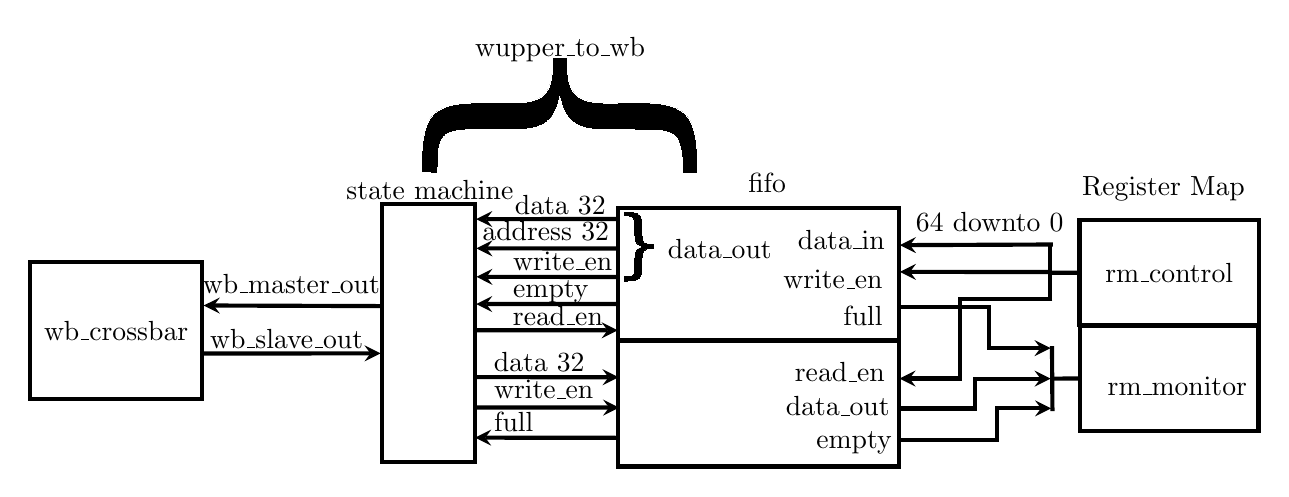
\begin{tikzpicture}
\pgftransformxscale{0.898485}
\pgftransformyscale{-0.898485}
\definecolor{dialinecolor}{rgb}{0.000000, 0.000000, 0.000000}
\pgfsetstrokecolor{dialinecolor}
\definecolor{dialinecolor}{rgb}{1.000000, 1.000000, 1.000000}
\pgfsetfillcolor{dialinecolor}
\definecolor{dialinecolor}{rgb}{1.000000, 1.000000, 1.000000}
\pgfsetfillcolor{dialinecolor}
\fill (74.997100\du,6.399620\du)--(74.997100\du,9.213650\du)--(79.807042\du,9.213650\du)--(79.807042\du,6.399620\du)--cycle;
\pgfsetlinewidth{0.100000\du}
\pgfsetdash{}{0pt}
\pgfsetdash{}{0pt}
\pgfsetmiterjoin
\definecolor{dialinecolor}{rgb}{0.000000, 0.000000, 0.000000}
\pgfsetstrokecolor{dialinecolor}
\draw (74.997100\du,6.399620\du)--(74.997100\du,9.213650\du)--(79.807042\du,9.213650\du)--(79.807042\du,6.399620\du)--cycle;
% setfont left to latex
\definecolor{dialinecolor}{rgb}{0.000000, 0.000000, 0.000000}
\pgfsetstrokecolor{dialinecolor}
\node[anchor=west] at (75.447100\du,8.001635\du){};
% setfont left to latex
\definecolor{dialinecolor}{rgb}{0.000000, 0.000000, 0.000000}
\pgfsetstrokecolor{dialinecolor}
\node[anchor=west] at (74.761700\du,5.544230\du){Register Map};
% setfont left to latex
\definecolor{dialinecolor}{rgb}{0.000000, 0.000000, 0.000000}
\pgfsetstrokecolor{dialinecolor}
\node[anchor=west] at (77.402071\du,7.806635\du){};
% setfont left to latex
\definecolor{dialinecolor}{rgb}{0.000000, 0.000000, 0.000000}
\pgfsetstrokecolor{dialinecolor}
\node[anchor=west] at (77.402071\du,8.606635\du){};
% setfont left to latex
\definecolor{dialinecolor}{rgb}{0.000000, 0.000000, 0.000000}
\pgfsetstrokecolor{dialinecolor}
\node[anchor=west] at (77.402071\du,7.806635\du){};
% setfont left to latex
\definecolor{dialinecolor}{rgb}{0.000000, 0.000000, 0.000000}
\pgfsetstrokecolor{dialinecolor}
\node[anchor=west] at (77.402071\du,7.806635\du){};
% setfont left to latex
\definecolor{dialinecolor}{rgb}{0.000000, 0.000000, 0.000000}
\pgfsetstrokecolor{dialinecolor}
\node at (77.402071\du,7.806635\du){rm\_control};
\definecolor{dialinecolor}{rgb}{1.000000, 1.000000, 1.000000}
\pgfsetfillcolor{dialinecolor}
\fill (62.624500\du,6.064760\du)--(62.624500\du,9.611836\du)--(70.163012\du,9.611836\du)--(70.163012\du,6.064760\du)--cycle;
\pgfsetlinewidth{0.100000\du}
\pgfsetdash{}{0pt}
\pgfsetdash{}{0pt}
\pgfsetmiterjoin
\definecolor{dialinecolor}{rgb}{0.000000, 0.000000, 0.000000}
\pgfsetstrokecolor{dialinecolor}
\draw (62.624500\du,6.064760\du)--(62.624500\du,9.611836\du)--(70.163012\du,9.611836\du)--(70.163012\du,6.064760\du)--cycle;
% setfont left to latex
\definecolor{dialinecolor}{rgb}{0.000000, 0.000000, 0.000000}
\pgfsetstrokecolor{dialinecolor}
\node[anchor=west] at (63.074500\du,8.033298\du){};
\definecolor{dialinecolor}{rgb}{1.000000, 1.000000, 1.000000}
\pgfsetfillcolor{dialinecolor}
\fill (56.286200\du,5.962470\du)--(56.286200\du,12.891096\du)--(58.780476\du,12.891096\du)--(58.780476\du,5.962470\du)--cycle;
\pgfsetlinewidth{0.100000\du}
\pgfsetdash{}{0pt}
\pgfsetdash{}{0pt}
\pgfsetmiterjoin
\definecolor{dialinecolor}{rgb}{0.000000, 0.000000, 0.000000}
\pgfsetstrokecolor{dialinecolor}
\draw (56.286200\du,5.962470\du)--(56.286200\du,12.891096\du)--(58.780476\du,12.891096\du)--(58.780476\du,5.962470\du)--cycle;
% setfont left to latex
\definecolor{dialinecolor}{rgb}{0.000000, 0.000000, 0.000000}
\pgfsetstrokecolor{dialinecolor}
\node[anchor=west] at (56.736200\du,9.621783\du){};
% setfont left to latex
\definecolor{dialinecolor}{rgb}{0.000000, 0.000000, 0.000000}
\pgfsetstrokecolor{dialinecolor}
\node[anchor=west] at (55.037200\du,5.582570\du){state machine};
% setfont left to latex
\definecolor{dialinecolor}{rgb}{0.000000, 0.000000, 0.000000}
\pgfsetstrokecolor{dialinecolor}
\node[anchor=west] at (65.815400\du,5.404550\du){fifo};
\pgfsetlinewidth{0.100000\du}
\pgfsetdash{}{0pt}
\pgfsetdash{}{0pt}
\pgfsetbuttcap
{
\definecolor{dialinecolor}{rgb}{0.000000, 0.000000, 0.000000}
\pgfsetfillcolor{dialinecolor}
% was here!!!
\pgfsetarrowsend{stealth}
\definecolor{dialinecolor}{rgb}{0.000000, 0.000000, 0.000000}
\pgfsetstrokecolor{dialinecolor}
\draw (74.282400\du,7.051110\du)--(70.180400\du,7.068340\du);
}
\pgfsetlinewidth{0.100000\du}
\pgfsetdash{}{0pt}
\pgfsetdash{}{0pt}
\pgfsetmiterjoin
\pgfsetbuttcap
{
\definecolor{dialinecolor}{rgb}{0.000000, 0.000000, 0.000000}
\pgfsetfillcolor{dialinecolor}
% was here!!!
\pgfsetarrowsend{stealth}
{\pgfsetcornersarced{\pgfpoint{0.000000\du}{0.000000\du}}\definecolor{dialinecolor}{rgb}{0.000000, 0.000000, 0.000000}
\pgfsetstrokecolor{dialinecolor}
\draw (74.268200\du,8.501990\du)--(71.796500\du,8.501990\du)--(71.796500\du,10.644300\du)--(70.171000\du,10.644300\du);
}}
\pgfsetlinewidth{0.100000\du}
\pgfsetdash{}{0pt}
\pgfsetdash{}{0pt}
\pgfsetmiterjoin
\pgfsetbuttcap
{
\definecolor{dialinecolor}{rgb}{0.000000, 0.000000, 0.000000}
\pgfsetfillcolor{dialinecolor}
% was here!!!
\pgfsetarrowsend{stealth}
{\pgfsetcornersarced{\pgfpoint{0.000000\du}{0.000000\du}}\definecolor{dialinecolor}{rgb}{0.000000, 0.000000, 0.000000}
\pgfsetstrokecolor{dialinecolor}
\draw (70.163012\du,8.725067\du)--(72.561200\du,8.725067\du)--(72.561200\du,9.828600\du)--(74.220100\du,9.828600\du);
}}
\pgfsetlinewidth{0.100000\du}
\pgfsetdash{}{0pt}
\pgfsetdash{}{0pt}
\pgfsetbuttcap
{
\definecolor{dialinecolor}{rgb}{0.000000, 0.000000, 0.000000}
\pgfsetfillcolor{dialinecolor}
% was here!!!
\definecolor{dialinecolor}{rgb}{0.000000, 0.000000, 0.000000}
\pgfsetstrokecolor{dialinecolor}
\draw (74.208600\du,7.063570\du)--(74.208600\du,8.528660\du);
}
\pgfsetlinewidth{0.100000\du}
\pgfsetdash{}{0pt}
\pgfsetdash{}{0pt}
\pgfsetbuttcap
{
\definecolor{dialinecolor}{rgb}{0.000000, 0.000000, 0.000000}
\pgfsetfillcolor{dialinecolor}
% was here!!!
\definecolor{dialinecolor}{rgb}{0.000000, 0.000000, 0.000000}
\pgfsetstrokecolor{dialinecolor}
\draw (74.258400\du,9.773260\du)--(74.270900\du,11.520000\du);
}
\pgfsetlinewidth{0.100000\du}
\pgfsetdash{}{0pt}
\pgfsetdash{}{0pt}
\pgfsetbuttcap
{
\definecolor{dialinecolor}{rgb}{0.000000, 0.000000, 0.000000}
\pgfsetfillcolor{dialinecolor}
% was here!!!
\definecolor{dialinecolor}{rgb}{0.000000, 0.000000, 0.000000}
\pgfsetstrokecolor{dialinecolor}
\draw (74.997100\du,7.806635\du)--(74.199300\du,7.807890\du);
}
% setfont left to latex
\definecolor{dialinecolor}{rgb}{0.000000, 0.000000, 0.000000}
\pgfsetstrokecolor{dialinecolor}
\node[anchor=west] at (67.143300\du,6.924590\du){data\_in};
% setfont left to latex
\definecolor{dialinecolor}{rgb}{0.000000, 0.000000, 0.000000}
\pgfsetstrokecolor{dialinecolor}
\node[anchor=west] at (66.754400\du,7.995430\du){   write\_en};
% setfont left to latex
\definecolor{dialinecolor}{rgb}{0.000000, 0.000000, 0.000000}
\pgfsetstrokecolor{dialinecolor}
\node[anchor=west] at (68.361600\du,8.966470\du){full};
% setfont left to latex
\definecolor{dialinecolor}{rgb}{0.000000, 0.000000, 0.000000}
\pgfsetstrokecolor{dialinecolor}
\node[anchor=west] at (57.745100\du,6.565980\du){};
\definecolor{dialinecolor}{rgb}{1.000000, 1.000000, 1.000000}
\pgfsetfillcolor{dialinecolor}
\fill (74.999400\du,9.241180\du)--(74.999400\du,12.047441\du)--(79.796900\du,12.047441\du)--(79.796900\du,9.241180\du)--cycle;
\pgfsetlinewidth{0.100000\du}
\pgfsetdash{}{0pt}
\pgfsetdash{}{0pt}
\pgfsetmiterjoin
\definecolor{dialinecolor}{rgb}{0.000000, 0.000000, 0.000000}
\pgfsetstrokecolor{dialinecolor}
\draw (74.999400\du,9.241180\du)--(74.999400\du,12.047441\du)--(79.796900\du,12.047441\du)--(79.796900\du,9.241180\du)--cycle;
% setfont left to latex
\definecolor{dialinecolor}{rgb}{0.000000, 0.000000, 0.000000}
\pgfsetstrokecolor{dialinecolor}
\node[anchor=west] at (75.449400\du,10.839311\du){rm\_monitor};
\definecolor{dialinecolor}{rgb}{1.000000, 1.000000, 1.000000}
\pgfsetfillcolor{dialinecolor}
\fill (62.631700\du,9.627140\du)--(62.631700\du,13.004695\du)--(70.149190\du,13.004695\du)--(70.149190\du,9.627140\du)--cycle;
\pgfsetlinewidth{0.100000\du}
\pgfsetdash{}{0pt}
\pgfsetdash{}{0pt}
\pgfsetmiterjoin
\definecolor{dialinecolor}{rgb}{0.000000, 0.000000, 0.000000}
\pgfsetstrokecolor{dialinecolor}
\draw (62.631700\du,9.627140\du)--(62.631700\du,13.004695\du)--(70.149190\du,13.004695\du)--(70.149190\du,9.627140\du)--cycle;
% setfont left to latex
\definecolor{dialinecolor}{rgb}{0.000000, 0.000000, 0.000000}
\pgfsetstrokecolor{dialinecolor}
\node[anchor=west] at (63.081700\du,11.510917\du){};
% setfont left to latex
\definecolor{dialinecolor}{rgb}{0.000000, 0.000000, 0.000000}
\pgfsetstrokecolor{dialinecolor}
\node[anchor=west] at (67.063200\du,10.479400\du){read\_en};
\pgfsetlinewidth{0.100000\du}
\pgfsetdash{}{0pt}
\pgfsetdash{}{0pt}
\pgfsetmiterjoin
\pgfsetbuttcap
{
\definecolor{dialinecolor}{rgb}{0.000000, 0.000000, 0.000000}
\pgfsetfillcolor{dialinecolor}
% was here!!!
\pgfsetarrowsend{stealth}
{\pgfsetcornersarced{\pgfpoint{0.000000\du}{0.000000\du}}\definecolor{dialinecolor}{rgb}{0.000000, 0.000000, 0.000000}
\pgfsetstrokecolor{dialinecolor}
\draw (70.181300\du,11.446200\du)--(72.201600\du,11.446200\du)--(72.201600\du,10.647100\du)--(74.221800\du,10.647100\du);
}}
\pgfsetlinewidth{0.100000\du}
\pgfsetdash{}{0pt}
\pgfsetdash{}{0pt}
\pgfsetmiterjoin
\pgfsetbuttcap
{
\definecolor{dialinecolor}{rgb}{0.000000, 0.000000, 0.000000}
\pgfsetfillcolor{dialinecolor}
% was here!!!
\pgfsetarrowsend{stealth}
{\pgfsetcornersarced{\pgfpoint{0.000000\du}{0.000000\du}}\definecolor{dialinecolor}{rgb}{0.000000, 0.000000, 0.000000}
\pgfsetstrokecolor{dialinecolor}
\draw (70.191800\du,12.297400\du)--(72.789700\du,12.297400\du)--(72.789700\du,11.445700\du)--(74.234700\du,11.445700\du);
}}
\pgfsetlinewidth{0.100000\du}
\pgfsetdash{}{0pt}
\pgfsetdash{}{0pt}
\pgfsetbuttcap
{
\definecolor{dialinecolor}{rgb}{0.000000, 0.000000, 0.000000}
\pgfsetfillcolor{dialinecolor}
% was here!!!
\pgfsetarrowsend{stealth}
\definecolor{dialinecolor}{rgb}{0.000000, 0.000000, 0.000000}
\pgfsetstrokecolor{dialinecolor}
\draw (74.177800\du,7.787760\du)--(70.181000\du,7.785130\du);
}
\pgfsetlinewidth{0.100000\du}
\pgfsetdash{}{0pt}
\pgfsetdash{}{0pt}
\pgfsetbuttcap
{
\definecolor{dialinecolor}{rgb}{0.000000, 0.000000, 0.000000}
\pgfsetfillcolor{dialinecolor}
% was here!!!
\definecolor{dialinecolor}{rgb}{0.000000, 0.000000, 0.000000}
\pgfsetstrokecolor{dialinecolor}
\draw (74.999400\du,10.644311\du)--(74.264650\du,10.646630\du);
}
% setfont left to latex
\definecolor{dialinecolor}{rgb}{0.000000, 0.000000, 0.000000}
\pgfsetstrokecolor{dialinecolor}
\node[anchor=west] at (66.393756\du,7.838298\du){};
\pgfsetlinewidth{0.000000\du}
\pgfsetdash{}{0pt}
\pgfsetmiterjoin
\pgfsetroundcap
\definecolor{dialinecolor}{rgb}{0.000000, 0.000000, 0.000000}
\pgfsetfillcolor{dialinecolor}
\pgfpathmoveto{\pgfpoint{57.794538\du}{5.136772\du}}
\pgfpathlineto{\pgfpoint{57.365556\du}{5.129235\du}}
\pgfpathlineto{\pgfpoint{57.355182\du}{4.877503\du}}
\pgfpathcurveto{\pgfpoint{57.357794\du}{4.234874\du}}{\pgfpoint{57.456422\du}{3.804078\du}}{\pgfpoint{57.651065\du}{3.585116\du}}
\pgfpathcurveto{\pgfpoint{57.843633\du}{3.362844\du}}{\pgfpoint{58.236804\du}{3.254506\du}}{\pgfpoint{58.826427\du}{3.253483\du}}
\pgfpathlineto{\pgfpoint{59.823492\du}{3.255066\du}}
\pgfpathcurveto{\pgfpoint{60.214779\du}{3.253974\du}}{\pgfpoint{60.483381\du}{3.182289\du}}{\pgfpoint{60.631374\du}{3.043322\du}}
\pgfpathcurveto{\pgfpoint{60.783909\du}{2.896893\du}}{\pgfpoint{60.862550\du}{2.640038\du}}{\pgfpoint{60.865219\du}{2.269448\du}}
\pgfpathlineto{\pgfpoint{60.863149\du}{2.030951\du}}
\pgfpathlineto{\pgfpoint{61.270591\du}{2.033557\du}}
\pgfpathlineto{\pgfpoint{61.272661\du}{2.272053\du}}
\pgfpathcurveto{\pgfpoint{61.269991\du}{2.642644\du}}{\pgfpoint{61.342066\du}{2.897167\du}}{\pgfpoint{61.494269\du}{3.036856\du}}
\pgfpathcurveto{\pgfpoint{61.647315\du}{3.185239\du}}{\pgfpoint{61.919482\du}{3.258884\du}}{\pgfpoint{62.316154\du}{3.259024\du}}
\pgfpathlineto{\pgfpoint{63.326454\du}{3.252303\du}}
\pgfpathcurveto{\pgfpoint{63.889995\du}{3.253810\du}}{\pgfpoint{64.269471\du}{3.366191\du}}{\pgfpoint{64.461573\du}{3.591522\du}}
\pgfpathcurveto{\pgfpoint{64.658217\du}{3.809391\du}}{\pgfpoint{64.757925\du}{4.240257\du}}{\pgfpoint{64.755313\du}{4.882886\du}}
\pgfpathlineto{\pgfpoint{64.765687\du}{5.134618\du}}
\pgfpathlineto{\pgfpoint{64.345010\du}{5.140317\du}}
\pgfpathlineto{\pgfpoint{64.347871\du}{4.880281\du}}
\pgfpathcurveto{\pgfpoint{64.340614\du}{4.515918\du}}{\pgfpoint{64.278077\du}{4.269246\du}}{\pgfpoint{64.164412\du}{4.146880\du}}
\pgfpathcurveto{\pgfpoint{64.054898\du}{4.031133\du}}{\pgfpoint{63.817961\du}{3.976888\du}}{\pgfpoint{63.453598\du}{3.984145\du}}
\pgfpathlineto{\pgfpoint{62.322363\du}{3.974513\du}}
\pgfpathcurveto{\pgfpoint{61.919074\du}{3.978525\du}}{\pgfpoint{61.627054\du}{3.917336\du}}{\pgfpoint{61.447536\du}{3.785562\du}}
\pgfpathcurveto{\pgfpoint{61.268862\du}{3.662481\du}}{\pgfpoint{61.140926\du}{3.429172\du}}{\pgfpoint{61.063729\du}{3.085634\du}}
\pgfpathcurveto{\pgfpoint{60.984826\du}{3.430271\du}}{\pgfpoint{60.854802\du}{3.664027\du}}{\pgfpoint{60.675732\du}{3.790213\du}}
\pgfpathcurveto{\pgfpoint{60.494586\du}{3.913090\du}}{\pgfpoint{60.202368\du}{3.976534\du}}{\pgfpoint{59.794926\du}{3.973928\du}}
\pgfpathlineto{\pgfpoint{58.671996\du}{3.977532\du}}
\pgfpathcurveto{\pgfpoint{58.301405\du}{3.974862\du}}{\pgfpoint{58.061350\du}{4.033248\du}}{\pgfpoint{57.951831\du}{4.152687\du}}
\pgfpathcurveto{\pgfpoint{57.840236\du}{4.268818\du}}{\pgfpoint{57.790142\du}{4.512374\du}}{\pgfpoint{57.797399\du}{4.876736\du}}
\pgfpathlineto{\pgfpoint{57.794538\du}{5.136772\du}}
\pgfusepath{fill}
\definecolor{dialinecolor}{rgb}{1.000000, 1.000000, 1.000000}
\pgfsetstrokecolor{dialinecolor}
\pgfpathmoveto{\pgfpoint{57.794538\du}{5.136772\du}}
\pgfpathlineto{\pgfpoint{57.365556\du}{5.129235\du}}
\pgfpathlineto{\pgfpoint{57.355182\du}{4.877503\du}}
\pgfpathcurveto{\pgfpoint{57.357794\du}{4.234874\du}}{\pgfpoint{57.456422\du}{3.804078\du}}{\pgfpoint{57.651065\du}{3.585116\du}}
\pgfpathcurveto{\pgfpoint{57.843633\du}{3.362844\du}}{\pgfpoint{58.236804\du}{3.254506\du}}{\pgfpoint{58.826427\du}{3.253483\du}}
\pgfpathlineto{\pgfpoint{59.823492\du}{3.255066\du}}
\pgfpathcurveto{\pgfpoint{60.214779\du}{3.253974\du}}{\pgfpoint{60.483381\du}{3.182289\du}}{\pgfpoint{60.631374\du}{3.043322\du}}
\pgfpathcurveto{\pgfpoint{60.783909\du}{2.896893\du}}{\pgfpoint{60.862550\du}{2.640038\du}}{\pgfpoint{60.865219\du}{2.269448\du}}
\pgfpathlineto{\pgfpoint{60.863149\du}{2.030951\du}}
\pgfpathlineto{\pgfpoint{61.270591\du}{2.033557\du}}
\pgfpathlineto{\pgfpoint{61.272661\du}{2.272053\du}}
\pgfpathcurveto{\pgfpoint{61.269991\du}{2.642644\du}}{\pgfpoint{61.342066\du}{2.897167\du}}{\pgfpoint{61.494269\du}{3.036856\du}}
\pgfpathcurveto{\pgfpoint{61.647315\du}{3.185239\du}}{\pgfpoint{61.919482\du}{3.258884\du}}{\pgfpoint{62.316154\du}{3.259024\du}}
\pgfpathlineto{\pgfpoint{63.326454\du}{3.252303\du}}
\pgfpathcurveto{\pgfpoint{63.889995\du}{3.253810\du}}{\pgfpoint{64.269471\du}{3.366191\du}}{\pgfpoint{64.461573\du}{3.591522\du}}
\pgfpathcurveto{\pgfpoint{64.658217\du}{3.809391\du}}{\pgfpoint{64.757925\du}{4.240257\du}}{\pgfpoint{64.755313\du}{4.882886\du}}
\pgfpathlineto{\pgfpoint{64.765687\du}{5.134618\du}}
\pgfpathlineto{\pgfpoint{64.345010\du}{5.140317\du}}
\pgfpathlineto{\pgfpoint{64.347871\du}{4.880281\du}}
\pgfpathcurveto{\pgfpoint{64.340614\du}{4.515918\du}}{\pgfpoint{64.278077\du}{4.269246\du}}{\pgfpoint{64.164412\du}{4.146880\du}}
\pgfpathcurveto{\pgfpoint{64.054898\du}{4.031133\du}}{\pgfpoint{63.817961\du}{3.976888\du}}{\pgfpoint{63.453598\du}{3.984145\du}}
\pgfpathlineto{\pgfpoint{62.322363\du}{3.974513\du}}
\pgfpathcurveto{\pgfpoint{61.919074\du}{3.978525\du}}{\pgfpoint{61.627054\du}{3.917336\du}}{\pgfpoint{61.447536\du}{3.785562\du}}
\pgfpathcurveto{\pgfpoint{61.268862\du}{3.662481\du}}{\pgfpoint{61.140926\du}{3.429172\du}}{\pgfpoint{61.063729\du}{3.085634\du}}
\pgfpathcurveto{\pgfpoint{60.984826\du}{3.430271\du}}{\pgfpoint{60.854802\du}{3.664027\du}}{\pgfpoint{60.675732\du}{3.790213\du}}
\pgfpathcurveto{\pgfpoint{60.494586\du}{3.913090\du}}{\pgfpoint{60.202368\du}{3.976534\du}}{\pgfpoint{59.794926\du}{3.973928\du}}
\pgfpathlineto{\pgfpoint{58.671996\du}{3.977532\du}}
\pgfpathcurveto{\pgfpoint{58.301405\du}{3.974862\du}}{\pgfpoint{58.061350\du}{4.033248\du}}{\pgfpoint{57.951831\du}{4.152687\du}}
\pgfpathcurveto{\pgfpoint{57.840236\du}{4.268818\du}}{\pgfpoint{57.790142\du}{4.512374\du}}{\pgfpoint{57.797399\du}{4.876736\du}}
\pgfpathlineto{\pgfpoint{57.794538\du}{5.136772\du}}
\pgfusepath{stroke}
% setfont left to latex
\definecolor{dialinecolor}{rgb}{0.000000, 0.000000, 0.000000}
\pgfsetstrokecolor{dialinecolor}
\node[anchor=west] at (58.544200\du,1.814590\du){wupper\_to\_wb};
\pgfsetlinewidth{0.100000\du}
\pgfsetdash{}{0pt}
\pgfsetdash{}{0pt}
\pgfsetbuttcap
{
\definecolor{dialinecolor}{rgb}{0.000000, 0.000000, 0.000000}
\pgfsetfillcolor{dialinecolor}
% was here!!!
\pgfsetarrowsend{stealth}
\definecolor{dialinecolor}{rgb}{0.000000, 0.000000, 0.000000}
\pgfsetstrokecolor{dialinecolor}
\draw (62.638300\du,6.367970\du)--(58.821500\du,6.370450\du);
}
\pgfsetlinewidth{0.100000\du}
\pgfsetdash{}{0pt}
\pgfsetdash{}{0pt}
\pgfsetbuttcap
{
\definecolor{dialinecolor}{rgb}{0.000000, 0.000000, 0.000000}
\pgfsetfillcolor{dialinecolor}
% was here!!!
\pgfsetarrowsend{stealth}
\definecolor{dialinecolor}{rgb}{0.000000, 0.000000, 0.000000}
\pgfsetstrokecolor{dialinecolor}
\draw (62.672900\du,7.159020\du)--(58.826800\du,7.153800\du);
}
\pgfsetlinewidth{0.100000\du}
\pgfsetdash{}{0pt}
\pgfsetdash{}{0pt}
\pgfsetbuttcap
{
\definecolor{dialinecolor}{rgb}{0.000000, 0.000000, 0.000000}
\pgfsetfillcolor{dialinecolor}
% was here!!!
\pgfsetarrowsend{stealth}
\definecolor{dialinecolor}{rgb}{0.000000, 0.000000, 0.000000}
\pgfsetstrokecolor{dialinecolor}
\draw (62.635600\du,7.922520\du)--(58.825900\du,7.917240\du);
}
\pgfsetlinewidth{0.100000\du}
\pgfsetdash{}{0pt}
\pgfsetdash{}{0pt}
\pgfsetbuttcap
{
\definecolor{dialinecolor}{rgb}{0.000000, 0.000000, 0.000000}
\pgfsetfillcolor{dialinecolor}
% was here!!!
\pgfsetarrowsend{stealth}
\definecolor{dialinecolor}{rgb}{0.000000, 0.000000, 0.000000}
\pgfsetstrokecolor{dialinecolor}
\draw (62.570200\du,8.645290\du)--(58.820600\du,8.648520\du);
}
\pgfsetlinewidth{0.100000\du}
\pgfsetdash{}{0pt}
\pgfsetdash{}{0pt}
\pgfsetbuttcap
{
\definecolor{dialinecolor}{rgb}{0.000000, 0.000000, 0.000000}
\pgfsetfillcolor{dialinecolor}
% was here!!!
\pgfsetarrowsend{stealth}
\definecolor{dialinecolor}{rgb}{0.000000, 0.000000, 0.000000}
\pgfsetstrokecolor{dialinecolor}
\draw (58.823100\du,9.349020\du)--(62.614400\du,9.352380\du);
}
% setfont left to latex
\definecolor{dialinecolor}{rgb}{0.000000, 0.000000, 0.000000}
\pgfsetstrokecolor{dialinecolor}
\node[anchor=west] at (59.556000\du,5.994200\du){data 32};
% setfont left to latex
\definecolor{dialinecolor}{rgb}{0.000000, 0.000000, 0.000000}
\pgfsetstrokecolor{dialinecolor}
\node[anchor=west] at (58.687100\du,6.680410\du){address 32};
% setfont left to latex
\definecolor{dialinecolor}{rgb}{0.000000, 0.000000, 0.000000}
\pgfsetstrokecolor{dialinecolor}
\node[anchor=west] at (59.509500\du,7.499060\du){write\_en};
% setfont left to latex
\definecolor{dialinecolor}{rgb}{0.000000, 0.000000, 0.000000}
\pgfsetstrokecolor{dialinecolor}
\node[anchor=west] at (59.509200\du,8.323520\du){empty};
% setfont left to latex
\definecolor{dialinecolor}{rgb}{0.000000, 0.000000, 0.000000}
\pgfsetstrokecolor{dialinecolor}
\node[anchor=west] at (59.503000\du,8.957970\du){read\_en};
\pgfsetlinewidth{0.100000\du}
\pgfsetdash{}{0pt}
\pgfsetdash{}{0pt}
\pgfsetbuttcap
{
\definecolor{dialinecolor}{rgb}{0.000000, 0.000000, 0.000000}
\pgfsetfillcolor{dialinecolor}
% was here!!!
\pgfsetarrowsend{stealth}
\definecolor{dialinecolor}{rgb}{0.000000, 0.000000, 0.000000}
\pgfsetstrokecolor{dialinecolor}
\draw (58.827400\du,10.606200\du)--(62.638900\du,10.611400\du);
}
\pgfsetlinewidth{0.100000\du}
\pgfsetdash{}{0pt}
\pgfsetdash{}{0pt}
\pgfsetbuttcap
{
\definecolor{dialinecolor}{rgb}{0.000000, 0.000000, 0.000000}
\pgfsetfillcolor{dialinecolor}
% was here!!!
\pgfsetarrowsend{stealth}
\definecolor{dialinecolor}{rgb}{0.000000, 0.000000, 0.000000}
\pgfsetstrokecolor{dialinecolor}
\draw (58.826400\du,11.419900\du)--(62.652700\du,11.423600\du);
}
\pgfsetlinewidth{0.100000\du}
\pgfsetdash{}{0pt}
\pgfsetdash{}{0pt}
\pgfsetbuttcap
{
\definecolor{dialinecolor}{rgb}{0.000000, 0.000000, 0.000000}
\pgfsetfillcolor{dialinecolor}
% was here!!!
\pgfsetarrowsend{stealth}
\definecolor{dialinecolor}{rgb}{0.000000, 0.000000, 0.000000}
\pgfsetstrokecolor{dialinecolor}
\draw (62.603000\du,12.234400\du)--(58.793300\du,12.229200\du);
}
% setfont left to latex
\definecolor{dialinecolor}{rgb}{0.000000, 0.000000, 0.000000}
\pgfsetstrokecolor{dialinecolor}
\node[anchor=west] at (58.990900\du,10.208900\du){data 32};
% setfont left to latex
\definecolor{dialinecolor}{rgb}{0.000000, 0.000000, 0.000000}
\pgfsetstrokecolor{dialinecolor}
\node[anchor=west] at (58.999700\du,10.941900\du){write\_en};
% setfont left to latex
\definecolor{dialinecolor}{rgb}{0.000000, 0.000000, 0.000000}
\pgfsetstrokecolor{dialinecolor}
\node[anchor=west] at (58.997400\du,11.809600\du){full};
\pgfsetlinewidth{0.000000\du}
\pgfsetdash{}{0pt}
\pgfsetmiterjoin
\pgfsetroundcap
\definecolor{dialinecolor}{rgb}{0.000000, 0.000000, 0.000000}
\pgfsetfillcolor{dialinecolor}
\pgfpathmoveto{\pgfpoint{62.796300\du}{7.921335\du}}
\pgfpathlineto{\pgfpoint{62.858800\du}{7.921335\du}}
\pgfpathcurveto{\pgfpoint{62.952550\du}{7.921335\du}}{\pgfpoint{63.007238\du}{7.905710\du}}{\pgfpoint{63.030675\du}{7.874460\du}}
\pgfpathcurveto{\pgfpoint{63.061925\du}{7.851023\du}}{\pgfpoint{63.077550\du}{7.796335\du}}{\pgfpoint{63.077550\du}{7.702585\du}}
\pgfpathlineto{\pgfpoint{63.077550\du}{7.421335\du}}
\pgfpathcurveto{\pgfpoint{63.077550\du}{7.319773\du}}{\pgfpoint{63.093175\du}{7.245554\du}}{\pgfpoint{63.124425\du}{7.202585\du}}
\pgfpathcurveto{\pgfpoint{63.163488\du}{7.163523\du}}{\pgfpoint{63.225988\du}{7.132273\du}}{\pgfpoint{63.311925\du}{7.108835\du}}
\pgfpathcurveto{\pgfpoint{63.225988\du}{7.089304\du}}{\pgfpoint{63.163488\du}{7.058054\du}}{\pgfpoint{63.124425\du}{7.015085\du}}
\pgfpathcurveto{\pgfpoint{63.093175\du}{6.964304\du}}{\pgfpoint{63.077550\du}{6.886179\du}}{\pgfpoint{63.077550\du}{6.780710\du}}
\pgfpathlineto{\pgfpoint{63.077550\du}{6.515085\du}}
\pgfpathcurveto{\pgfpoint{63.077550\du}{6.421335\du}}{\pgfpoint{63.061925\du}{6.358835\du}}{\pgfpoint{63.030675\du}{6.327585\du}}
\pgfpathcurveto{\pgfpoint{63.007238\du}{6.296335\du}}{\pgfpoint{62.952550\du}{6.280710\du}}{\pgfpoint{62.858800\du}{6.280710\du}}
\pgfpathlineto{\pgfpoint{62.796300\du}{6.280710\du}}
\pgfpathlineto{\pgfpoint{62.796300\du}{6.186960\du}}
\pgfpathlineto{\pgfpoint{62.858800\du}{6.186960\du}}
\pgfpathcurveto{\pgfpoint{63.022863\du}{6.186960\du}}{\pgfpoint{63.132238\du}{6.214304\du}}{\pgfpoint{63.186925\du}{6.265085\du}}
\pgfpathcurveto{\pgfpoint{63.237706\du}{6.308054\du}}{\pgfpoint{63.265050\du}{6.401804\du}}{\pgfpoint{63.265050\du}{6.546335\du}}
\pgfpathlineto{\pgfpoint{63.265050\du}{6.796335\du}}
\pgfpathcurveto{\pgfpoint{63.265050\du}{6.890085\du}}{\pgfpoint{63.280675\du}{6.960398\du}}{\pgfpoint{63.311925\du}{6.999460\du}}
\pgfpathcurveto{\pgfpoint{63.350988\du}{7.030710\du}}{\pgfpoint{63.421300\du}{7.046335\du}}{\pgfpoint{63.515050\du}{7.046335\du}}
\pgfpathlineto{\pgfpoint{63.561925\du}{7.046335\du}}
\pgfpathlineto{\pgfpoint{63.561925\du}{7.155710\du}}
\pgfpathlineto{\pgfpoint{63.515050\du}{7.155710\du}}
\pgfpathcurveto{\pgfpoint{63.421300\du}{7.155710\du}}{\pgfpoint{63.350988\du}{7.179148\du}}{\pgfpoint{63.311925\du}{7.218210\du}}
\pgfpathcurveto{\pgfpoint{63.280675\du}{7.249460\du}}{\pgfpoint{63.265050\du}{7.319773\du}}{\pgfpoint{63.265050\du}{7.421335\du}}
\pgfpathlineto{\pgfpoint{63.265050\du}{7.671335\du}}
\pgfpathcurveto{\pgfpoint{63.265050\du}{7.815866\du}}{\pgfpoint{63.237706\du}{7.909616\du}}{\pgfpoint{63.186925\du}{7.952585\du}}
\pgfpathcurveto{\pgfpoint{63.132238\du}{8.003366\du}}{\pgfpoint{63.022863\du}{8.030710\du}}{\pgfpoint{62.858800\du}{8.030710\du}}
\pgfpathlineto{\pgfpoint{62.796300\du}{8.030710\du}}
\pgfpathlineto{\pgfpoint{62.796300\du}{7.921335\du}}
\pgfusepath{fill}
\definecolor{dialinecolor}{rgb}{0.000000, 0.000000, 0.000000}
\pgfsetstrokecolor{dialinecolor}
\pgfpathmoveto{\pgfpoint{62.796300\du}{7.921335\du}}
\pgfpathlineto{\pgfpoint{62.858800\du}{7.921335\du}}
\pgfpathcurveto{\pgfpoint{62.952550\du}{7.921335\du}}{\pgfpoint{63.007238\du}{7.905710\du}}{\pgfpoint{63.030675\du}{7.874460\du}}
\pgfpathcurveto{\pgfpoint{63.061925\du}{7.851023\du}}{\pgfpoint{63.077550\du}{7.796335\du}}{\pgfpoint{63.077550\du}{7.702585\du}}
\pgfpathlineto{\pgfpoint{63.077550\du}{7.421335\du}}
\pgfpathcurveto{\pgfpoint{63.077550\du}{7.319773\du}}{\pgfpoint{63.093175\du}{7.245554\du}}{\pgfpoint{63.124425\du}{7.202585\du}}
\pgfpathcurveto{\pgfpoint{63.163488\du}{7.163523\du}}{\pgfpoint{63.225988\du}{7.132273\du}}{\pgfpoint{63.311925\du}{7.108835\du}}
\pgfpathcurveto{\pgfpoint{63.225988\du}{7.089304\du}}{\pgfpoint{63.163488\du}{7.058054\du}}{\pgfpoint{63.124425\du}{7.015085\du}}
\pgfpathcurveto{\pgfpoint{63.093175\du}{6.964304\du}}{\pgfpoint{63.077550\du}{6.886179\du}}{\pgfpoint{63.077550\du}{6.780710\du}}
\pgfpathlineto{\pgfpoint{63.077550\du}{6.515085\du}}
\pgfpathcurveto{\pgfpoint{63.077550\du}{6.421335\du}}{\pgfpoint{63.061925\du}{6.358835\du}}{\pgfpoint{63.030675\du}{6.327585\du}}
\pgfpathcurveto{\pgfpoint{63.007238\du}{6.296335\du}}{\pgfpoint{62.952550\du}{6.280710\du}}{\pgfpoint{62.858800\du}{6.280710\du}}
\pgfpathlineto{\pgfpoint{62.796300\du}{6.280710\du}}
\pgfpathlineto{\pgfpoint{62.796300\du}{6.186960\du}}
\pgfpathlineto{\pgfpoint{62.858800\du}{6.186960\du}}
\pgfpathcurveto{\pgfpoint{63.022863\du}{6.186960\du}}{\pgfpoint{63.132238\du}{6.214304\du}}{\pgfpoint{63.186925\du}{6.265085\du}}
\pgfpathcurveto{\pgfpoint{63.237706\du}{6.308054\du}}{\pgfpoint{63.265050\du}{6.401804\du}}{\pgfpoint{63.265050\du}{6.546335\du}}
\pgfpathlineto{\pgfpoint{63.265050\du}{6.796335\du}}
\pgfpathcurveto{\pgfpoint{63.265050\du}{6.890085\du}}{\pgfpoint{63.280675\du}{6.960398\du}}{\pgfpoint{63.311925\du}{6.999460\du}}
\pgfpathcurveto{\pgfpoint{63.350988\du}{7.030710\du}}{\pgfpoint{63.421300\du}{7.046335\du}}{\pgfpoint{63.515050\du}{7.046335\du}}
\pgfpathlineto{\pgfpoint{63.561925\du}{7.046335\du}}
\pgfpathlineto{\pgfpoint{63.561925\du}{7.155710\du}}
\pgfpathlineto{\pgfpoint{63.515050\du}{7.155710\du}}
\pgfpathcurveto{\pgfpoint{63.421300\du}{7.155710\du}}{\pgfpoint{63.350988\du}{7.179148\du}}{\pgfpoint{63.311925\du}{7.218210\du}}
\pgfpathcurveto{\pgfpoint{63.280675\du}{7.249460\du}}{\pgfpoint{63.265050\du}{7.319773\du}}{\pgfpoint{63.265050\du}{7.421335\du}}
\pgfpathlineto{\pgfpoint{63.265050\du}{7.671335\du}}
\pgfpathcurveto{\pgfpoint{63.265050\du}{7.815866\du}}{\pgfpoint{63.237706\du}{7.909616\du}}{\pgfpoint{63.186925\du}{7.952585\du}}
\pgfpathcurveto{\pgfpoint{63.132238\du}{8.003366\du}}{\pgfpoint{63.022863\du}{8.030710\du}}{\pgfpoint{62.858800\du}{8.030710\du}}
\pgfpathlineto{\pgfpoint{62.796300\du}{8.030710\du}}
\pgfpathlineto{\pgfpoint{62.796300\du}{7.921335\du}}
\pgfusepath{stroke}
% setfont left to latex
\definecolor{dialinecolor}{rgb}{0.000000, 0.000000, 0.000000}
\pgfsetstrokecolor{dialinecolor}
\node[anchor=west] at (63.715200\du,7.159930\du){data\_out};
% setfont left to latex
\definecolor{dialinecolor}{rgb}{0.000000, 0.000000, 0.000000}
\pgfsetstrokecolor{dialinecolor}
\node[anchor=west] at (70.365000\du,6.433490\du){64 downto 0};
% setfont left to latex
\definecolor{dialinecolor}{rgb}{0.000000, 0.000000, 0.000000}
\pgfsetstrokecolor{dialinecolor}
\node[anchor=west] at (66.875100\du,11.385800\du){data\_out};
% setfont left to latex
\definecolor{dialinecolor}{rgb}{0.000000, 0.000000, 0.000000}
\pgfsetstrokecolor{dialinecolor}
\node[anchor=west] at (67.694700\du,12.356800\du){empty};
\pgfsetlinewidth{0.100000\du}
\pgfsetdash{}{0pt}
\pgfsetdash{}{0pt}
\pgfsetbuttcap
{
\definecolor{dialinecolor}{rgb}{0.000000, 0.000000, 0.000000}
\pgfsetfillcolor{dialinecolor}
% was here!!!
\pgfsetarrowsend{stealth}
\definecolor{dialinecolor}{rgb}{0.000000, 0.000000, 0.000000}
\pgfsetstrokecolor{dialinecolor}
\draw (56.249100\du,8.702340\du)--(51.515200\du,8.686270\du);
}
\pgfsetlinewidth{0.100000\du}
\pgfsetdash{}{0pt}
\pgfsetdash{}{0pt}
\pgfsetbuttcap
{
\definecolor{dialinecolor}{rgb}{0.000000, 0.000000, 0.000000}
\pgfsetfillcolor{dialinecolor}
% was here!!!
\pgfsetarrowsend{stealth}
\definecolor{dialinecolor}{rgb}{0.000000, 0.000000, 0.000000}
\pgfsetstrokecolor{dialinecolor}
\draw (51.518100\du,9.973020\du)--(56.256400\du,9.970370\du);
}
% setfont left to latex
\definecolor{dialinecolor}{rgb}{0.000000, 0.000000, 0.000000}
\pgfsetstrokecolor{dialinecolor}
\node[anchor=west] at (51.188600\du,8.097880\du){wb\_master\_out};
% setfont left to latex
\definecolor{dialinecolor}{rgb}{0.000000, 0.000000, 0.000000}
\pgfsetstrokecolor{dialinecolor}
\node[anchor=west] at (51.381900\du,9.568770\du){wb\_slave\_out};
\pgfsetlinewidth{0.100000\du}
\pgfsetdash{}{0pt}
\pgfsetdash{}{0pt}
\pgfsetmiterjoin
\definecolor{dialinecolor}{rgb}{1.000000, 1.000000, 1.000000}
\pgfsetfillcolor{dialinecolor}
\fill (46.851400\du,7.510990\du)--(46.851400\du,11.186237\du)--(51.464058\du,11.186237\du)--(51.464058\du,7.510990\du)--cycle;
\definecolor{dialinecolor}{rgb}{0.000000, 0.000000, 0.000000}
\pgfsetstrokecolor{dialinecolor}
\draw (46.851400\du,7.510990\du)--(46.851400\du,11.186237\du)--(51.464058\du,11.186237\du)--(51.464058\du,7.510990\du)--cycle;
% setfont left to latex
\definecolor{dialinecolor}{rgb}{0.000000, 0.000000, 0.000000}
\pgfsetstrokecolor{dialinecolor}
\node[anchor=west] at (46.930700\du,9.357270\du){wb\_crossbar};
\end{tikzpicture}

	\caption{Block diagram of Wupper to Wishbone}
	\label{fig:wupper_to_wishbone}
\end{figure}
\end{flushleft}

\newpage
